\documentclass{article}
\usepackage{booktabs}
\usepackage{upgreek}
\usepackage{enumerate}

\usepackage[english]{babel}
\usepackage[letterpaper,top=2cm,bottom=2cm,left=3cm,right=3cm,marginparwidth=1.75cm]{geometry}
\usepackage{amsmath}
\usepackage{graphicx}
\usepackage[colorlinks=true, allcolors=blue]{hyperref}

\title{Study of Electron Transverse Emittance Mismatch in the EIC Swap-Out Injection Scheme}
\author{Derong Xu}

\begin{document}
\maketitle

\begin{abstract}
This study examines the effect of electron emittance mismatch 
on proton emittance growth in the EIC swap-out injection. 
Strong-strong simulations show negligible growth for electron 
charge of 7 and 14 nC, but significant growth at 28 nC 
when electron emittance is much smaller than design values.
\end{abstract}
%%%%%%%%%%%%%%%%%%%%%%%%%%%%%%%%%%%%%%%%%%%%%%%%%%%%%%%%%%%%%%%
\section{Introduction}
The Electron-Ion Collider (EIC) is designed to achieve a high peak luminosity of 
$10^{34}~\mathrm{cm}^{-2}\mathrm{s}^{-1}$ through collisions of polarized electron and 
proton beams. The Electron Storage Ring (ESR) is expected to 
deliver high-charge electron bunches of up to $28~\mathrm{nC}$.
The ESR lattice is engineered to provide a dynamic aperture of $10\sigma$ in all three 
planes. Due to the limited polarization lifetime, frequent electron bunch replacement 
is required. The swap-out injection scheme offers an efficient solution to meet these 
demands, while accommodating the small dynamic aperture. The Rapid Cycling Synchrotron 
(RCS) is responsible for electron accumulation, acceleration, and injection to the ESR.

However, the design emittances of the RCS and ESR differ significantly. 
In the RCS, the vertical emittance is nearly zero to suppress vertical intrinsic 
spin resonances. In contrast, the ESR maintains a finite vertical emittance to 
match the proton beam size at the interaction point (IP). 
Although the electron beam can be manipulated during transport from the RCS to 
the ESR, maintaining precise control over the resulting emittance is challenging.
This emittance mismatch during electron injection can lead to proton emittance growth.

An alternative injection scheme involves injecting electron bunches directly from the 
LINAC into the ESR, eliminating the need for the RCS. This approach meets the Phase I 
goals, where the ESR only needs to provide $5/10~\mathrm{GeV}$ electron bunches with 
a maximum charge of $7~\mathrm{nC}$ \cite{EICMACReview202409:Sergei} . In Phase II, where a $28~\mathrm{nC}$ electron 
bunch is required, multiple electron bunches can be injected into the same ESR bucket. 
Off-momentum injection can be employed to minimize electron emittance blow-up, 
making this accumulation scheme feasible. Our previous study indicates that 
the accumulation scheme is a viable option \cite{xu:ipac2024-mopc72}.

The electron bunch from the LINAC also differs from the ESR design value. 
In this note, we apply the strong-strong simulation method to study proton 
emittance growth during the swap-out injection for electron bunch charges of $7$, 
$14$, and $28~\mathrm{nC}$, respectively. The electron injection emittance spans 
a wide range to account for both LINAC and RCS cases. The accumulation scenario 
with significant emittance mismatch will be revisited in future studies.
%%%%%%%%%%%%%%%%%%%%%%%%%%%%%%%%%%%%%%%%%%%%%%%%%%%%%%%%%%%%%%%
\section{Method}
To model the distribution evolution of both the electron and proton beams, 
a self-consistent simulation is required. Accordingly, we employ 
the strong-strong simulation method. The beam parameters used in the simulation 
are presented in Table~\ref{tab:SimulationParameters}. 

\begin{table}
  \centering
  \caption{Beam parameters used in strong-strong simulation. The columns ``Proton 
  design'' and ``Electron design'' are directly taken from EIC-CDR 
  \cite{willeke2021electron}. The ``Electron input'' is what we actually use in
  the simulation. Without beam-beam interaction, the electron beam parameters
  will evolve toward the ``Electron design'' parameter.
  ``H'' stands for horizontal and ``V'' denotes vertical below.
  Parameters marked in red as ``TBD'' indicate values that were scanned during 
  the simulation.\\}
  \begin{tabular}{lcccc}
   \toprule
    Parameter & Unit & Proton design & Electron design & Electron input\\
    \hline
    Circumference & $\mathrm{m}$ & $3834$ & $3834$ & $3834$ \\
    Energy & $\mathrm{GeV}$ & $275$ & $10$ & $10$\\
    Particles per bunch & $10^{11}$ & $0.688$ & $1.72$ & $1.72$\\
    Half crossing angle & $\mathrm{mrad}$ & $12.5$ & $12.5$ & $12.5$\\
    Crab cavity frequency & $\mathrm{MHz}$ & $200.0/400.0$ & $400.0$ & $400.0$\\
    $\beta_x^*/\beta_y^*$ & $\mathrm{cm}$ & $80.0/7.20$ & $55.0/5.60$ & $55.0/5.60$\\
    RMS emittance (H/V) & $\mathrm{nm\cdot rad}$ & $11.3/1.00$ & $20.4/1.6$ & \textcolor{red}{TBD}\\
    RMS bunch size (H/V) & $\mathrm{\upmu m}$ & $95.0/8.5$ & $106/9.5$ & \textcolor{red}{TBD}\\
    RMS bunch length & $\mathrm{cm}$ & $6.0$ & $0.7$ & $0.09$\\
    RMS energy spread & $10^{-4}$ & $6.6$ & $5.5$ & $20.0$\\
    Transverse fractional tune (H/V) & - & $0.228/0.210$ & $0.08/0.14$ & $0.08/0.14$\\
    Synchrotron tune  & - & $-0.010$ & $-0.069$ & $-0.069$\\
    Transverse damping time & turns & $\infty$ & $4000$ & $4000$\\
    Longitudinal damping time & turns & $\infty$ & $2000$ & $2000$\\
    Chromaticity (H/V) & - & $2/2$ & $1/1$ & $1/1$\\
  \bottomrule
  \end{tabular}
  \label{tab:SimulationParameters}
\end{table}

The horizontal emittance of the electron beam is scanned from $5~\mathrm{nm}$ to 
$23~\mathrm{nm}$ in steps of $2~\mathrm{nm}$. The vertical emittance is scanned 
from $0.5~\mathrm{nm}$ to $5.0~\mathrm{nm}$, with a step size of $0.5~\mathrm{nm}$. 
The injected electron bunches are assumed to match the ESR optics, and their initial 
beam sizes are determined based on the scanned emittance and beam optics. 
The initial proton beam follows a perfect Gaussian distribution and begins interacting 
with the electron beam from the 1st turn. After $50,000$ turns, the electron bunch 
is swapped out and replaced with a fresh one, allowing the HSR bunch to 
continue interaction with the newly injected electron bunch.

The strong-strong simulation is influenced by numerical noise, which varies based on 
the model parameters. The chosen model parameters are listed in Table \ref{tab:model}.
The ratio of macro particles is set equal to the ratio of bunch intensities, 
following our previous study. To reduce computation time, we also reduce the 
number of longitudinal slices and transverse grids.
\begin{table}
    \centering
    \caption{Model parameters during the strong-strong simulation\\}
    \begin{tabular}{lcc}
    \toprule
    Model parameter & Proton beam & Electron beam\\
    \midrule
    Number of macro particles & $512,000$ & $1,280,000$\\
    Number of longitudinal slices & $11$ & $11$\\
    Number of transverse grids & \multicolumn{2}{c}{$64\times 64$}\\
    \bottomrule
    \end{tabular}
    \label{tab:model}
\end{table}

%%%%%%%%%%%%%%%%%%%%%%%%%%%%%%%%%%%%%%%%%%%%%%%%%%%%%%%%%%%%%%%
\section{Result}
A typical tracking result is shown in Figure~\ref{fig:ssTrackingExample}.
At 50,000-th turns, following the replacement of the electron bunch, a slight jump 
in the proton vertical emittance is observed. This emittance jump must be 
carefully controlled to remain small; otherwise, the flat hadron beam profile 
may be compromised.
More tracking results are available at \href{https://github.com/xud929/ESR_injection_swapOut/tree/main/pic}{Github repository}.
\begin{figure}
    \centering
    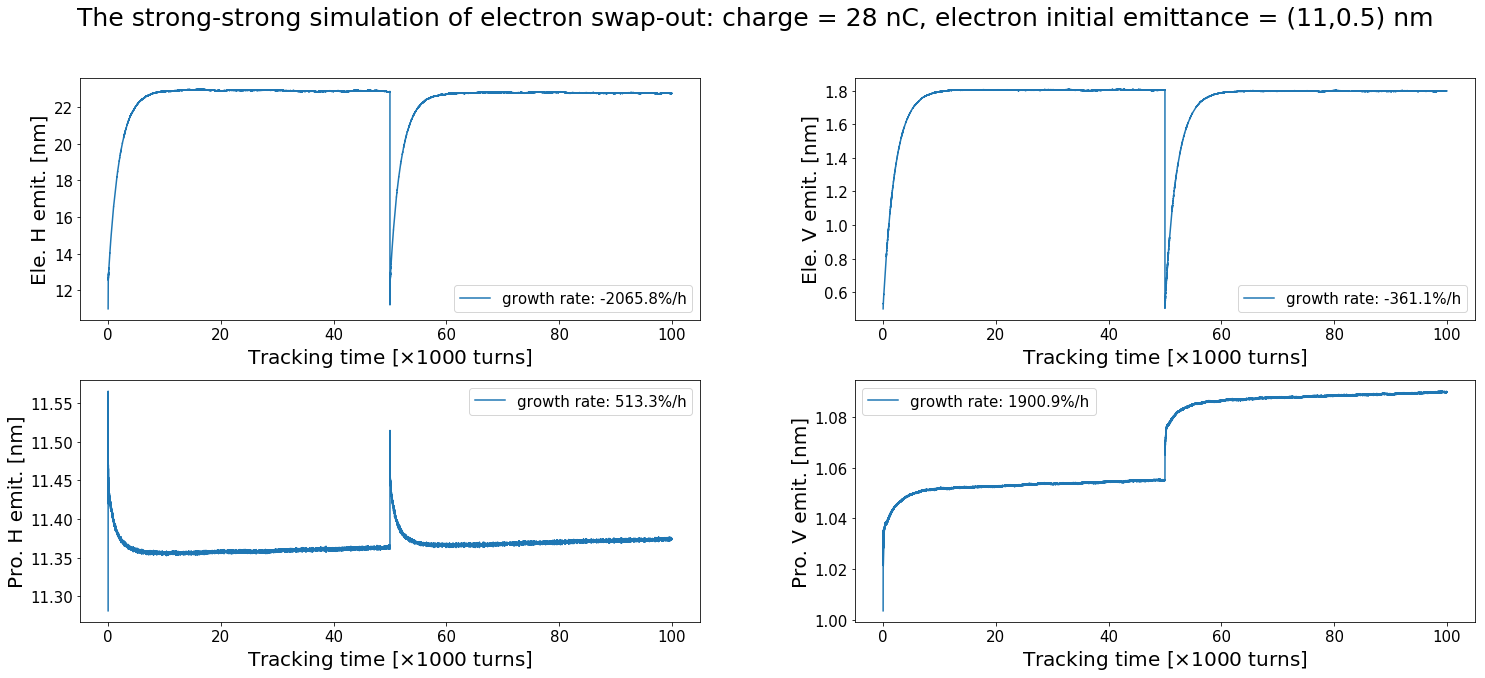
\includegraphics[width=0.99\textwidth]{pic/28nC_track/11_0.5.png}
    \caption{Electron (top) and proton (bottom) emittance evolution in strong-strong simulation.}
    \label{fig:ssTrackingExample}
\end{figure}

Figure~\ref{fig:protonEmittanceJump} presents the proton horizontal and vertical 
emittance jumps for varying initial electron emittances and electron charges. 
Different colors represent the percentage increase in emittance per injection.
The emittance increase is calculated as follows:
\begin{enumerate}[(1)]
    \item The tracking data between 40,000 and 41,000 turns are averaged to obtain $\epsilon_1$
    \item The tracking data between 90,000 and 91,000 turns are averaged to obtain $\epsilon_2$
    \item The relative emittance growth per injection is normalized using
    \begin{displaymath}
    \frac{\Delta \epsilon}{\epsilon_0}=\frac{\epsilon_2-\epsilon_1}{\epsilon_0}
    \end{displaymath}
    where $\epsilon_0$ is the proton design value shown in Table \ref{tab:SimulationParameters}.
\end{enumerate}

From Figure~\ref{fig:protonEmittanceJump}, it is evident that the emittance jump is 
negligible for electron charges of $7~\mathrm{nC}$ or $14~\mathrm{nC}$. 
However, for $28~\mathrm{nC}$, with smaller injected 
emittances (e.g. $\epsilon_x=5~\mathrm{nm},~\epsilon_y=0.5~\mathrm{nm}$), 
the vertical emittance jump reaches as high as $9.2\%$ per injection, which is 
unacceptably large. Increasing the injected horizontal or vertical electron emittance 
helps reduce the emittance jump. When the injected electron emittance is matched to 
the design values ($\epsilon_x\sim 20~\mathrm{nm},\epsilon_y\sim 2~\mathrm{nm}$), 
the proton emittance jump is minimized.

\begin{figure}
    \centering
    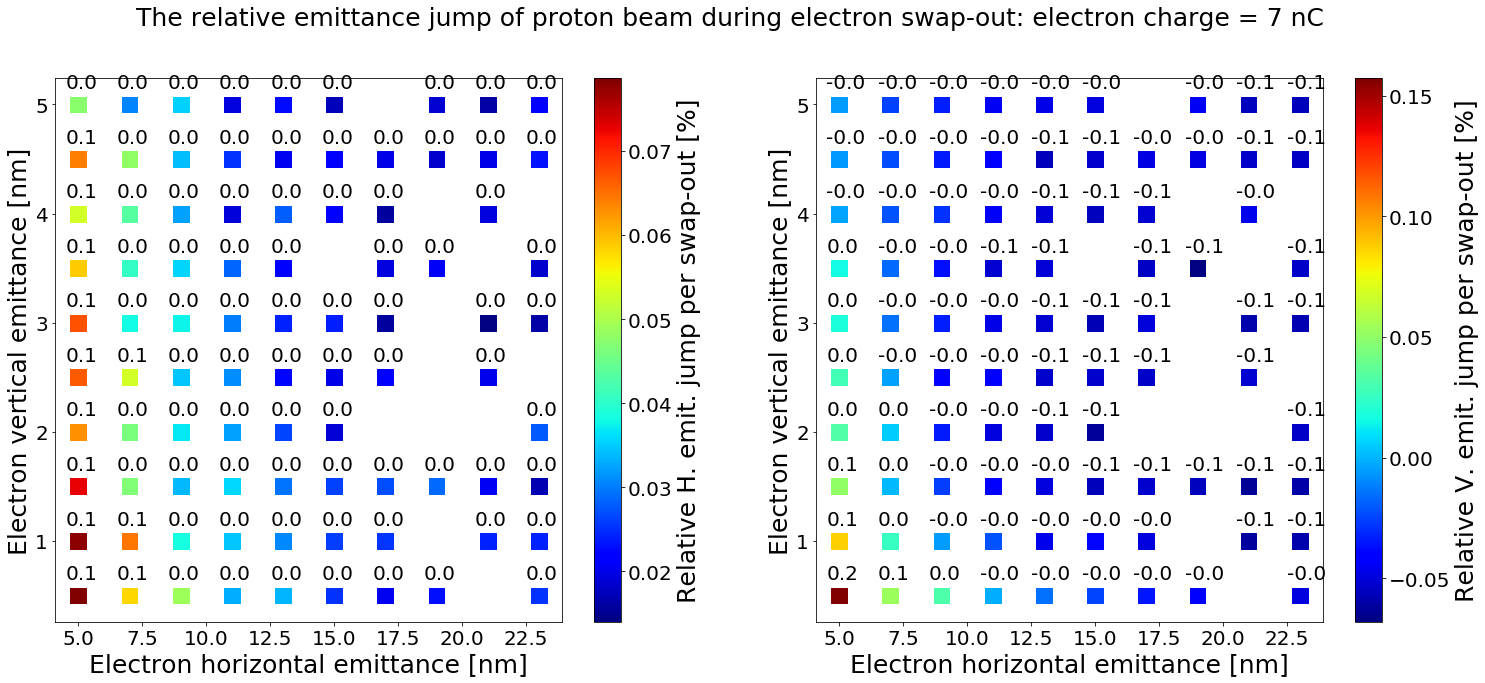
\includegraphics[width=0.99\textwidth]{pic/07.png}
    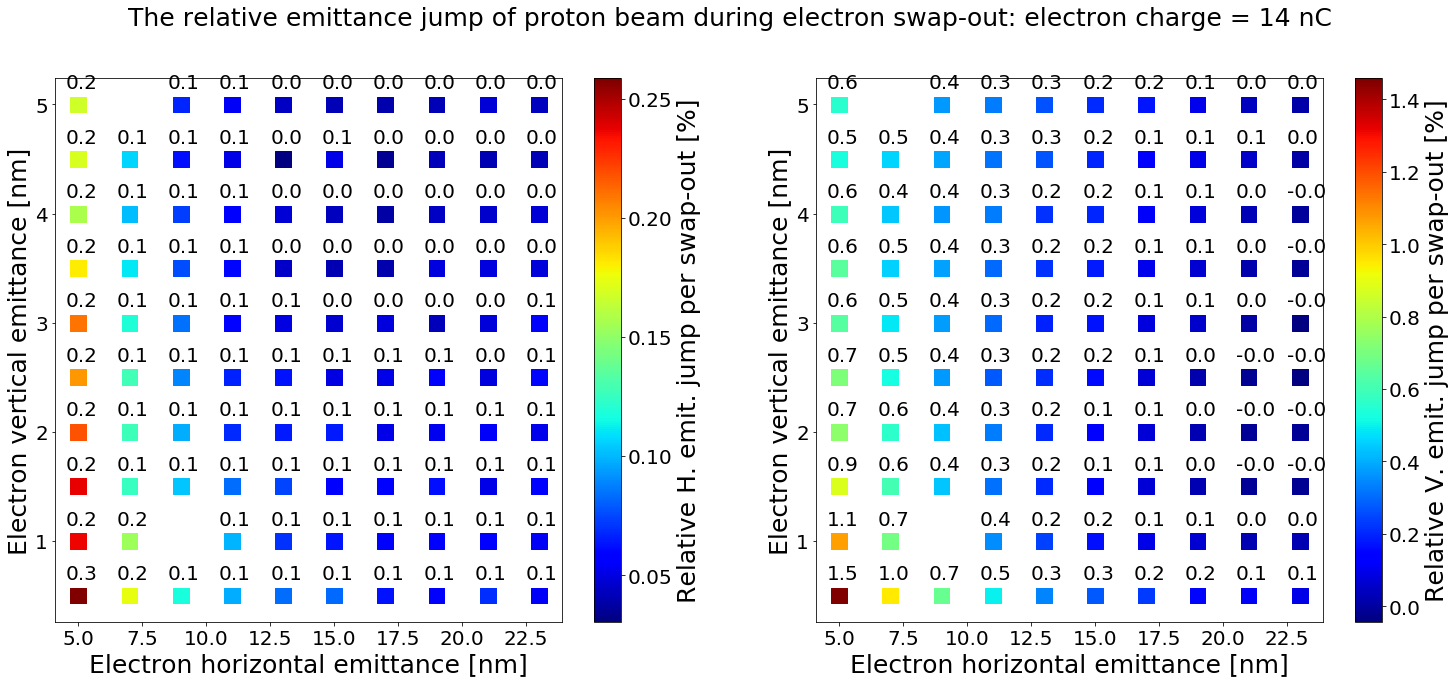
\includegraphics[width=0.99\textwidth]{pic/14.png}
    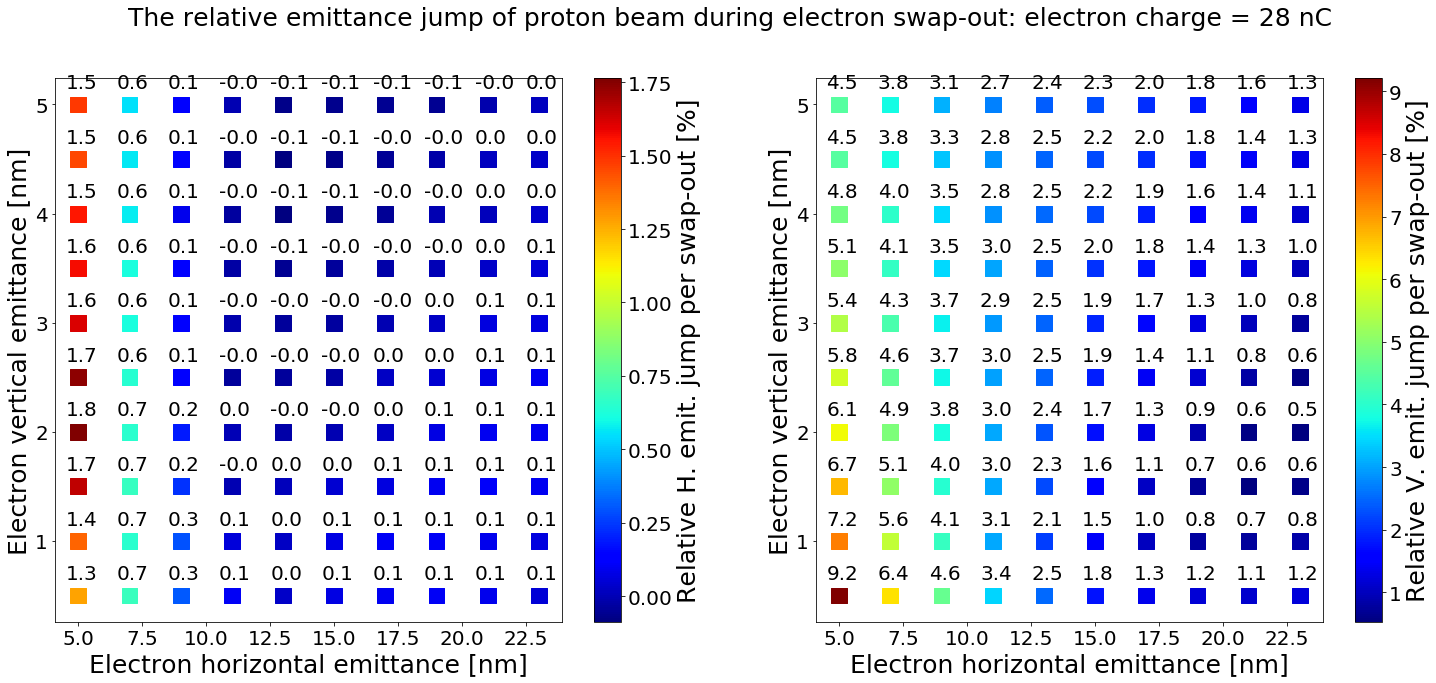
\includegraphics[width=0.99\textwidth]{pic/28.png}
    \caption{Relative proton emittance growth per injection. Empty blocks indicate that the simulation was terminated accidentally, resulting in insufficient tracking data.}
    \label{fig:protonEmittanceJump}
\end{figure}

%%%%%%%%%%%%%%%%%%%%%%%%%%%%%%%%%%%%%%%%%%%%%%%%%%%%%%%%%%%%%%%
\section{Discussion}
In addition to the emittance jump observed during the swap-out 
process, there is a gradual vertical emittance decrease at 
$7 ~\mathrm{nC}$ or $14~\mathrm{nC}$. This behavior 
contrasts with the case of $28~\mathrm{nC}$, where both 
horizontal and vertical growth rates are positive.

Figure~\ref{fig:compareCharge} compares the emittance tracking
result for different electron charge. The emittance growth 
rate is fitted by last $30\%$ tracking data, which is $30,000$
turns. As shown in this figure, the proton vertical growth
rate is negative for $7~\mathrm{nC}$ or $14~\mathrm{nC}$.

One possible explanation is that the beam-beam kick is too 
weak, and the tracking duration is not long enough for the 
proton beam distribution to reach equilibrium. Another factor 
could be that the growth rate in the simulation is sensitive 
to the model parameters, as we also observed in a previous 
study regarding the impact of numerical noise on proton 
emittance growth in strong-strong simulations \cite{xu:beamDynamicsWorkshop}. 

Figure~\ref{fig:compareModel} presents the strong-strong 
tracking results using different model parameters. 
The beam parameters are set according to the EIC design 
values listed in Table~\ref{tab:SimulationParameters}
Models A, B, and C are detailed in Tables~\ref{tab:model},
,\ref{tab:modelB}, and \ref{tab:modelC}, respectively.
The results clearly demonstrate that the proton growth rate 
in strong-strong simulations is dependent on the model 
parameters, with the vertical growth rates varying from 
negative to positive.

\begin{figure}
    \centering
    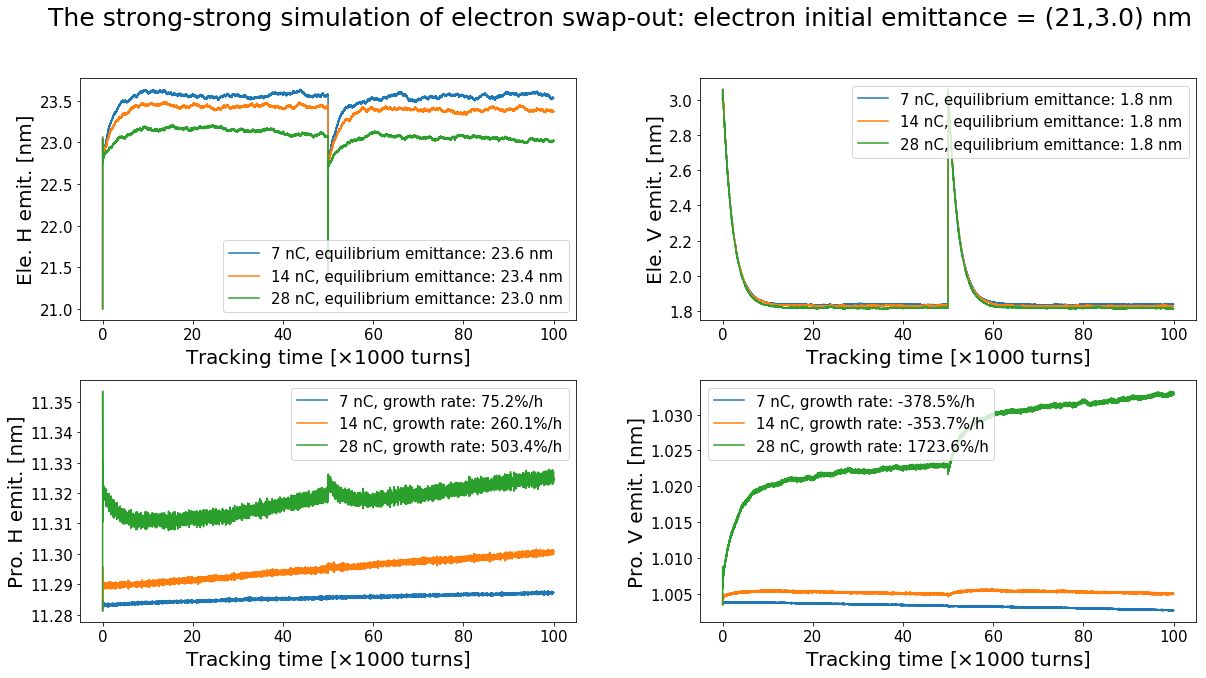
\includegraphics[width=0.99\textwidth]{pic/compareCharge.png}
    \caption{The vertical emittance growth rate of proton beam are negative for $7~\mathrm{nC}$ or $14~\mathrm{nC}$.}
    \label{fig:compareCharge}
\end{figure}

\begin{figure}
    \centering
    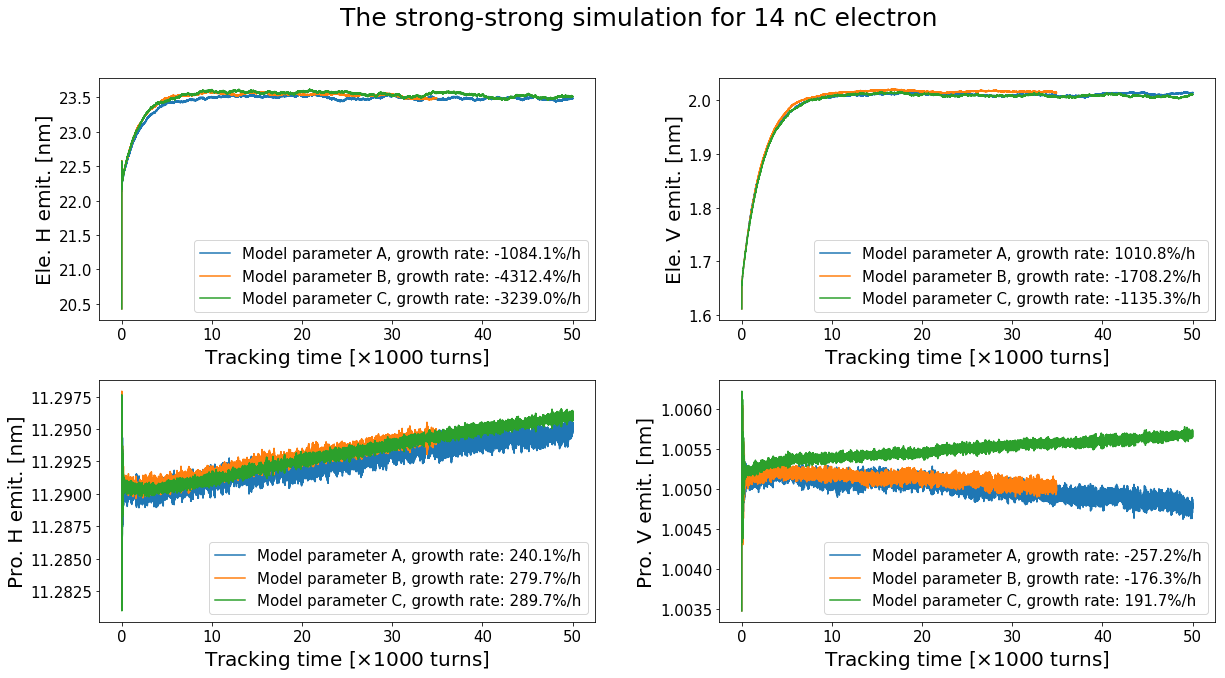
\includegraphics[width=0.99\textwidth]{pic/compareModel.png}
    \caption{The vertical emittance growth rate in strong-strong simulation depends on model parameters. Models A, B, and C are detailed in Tables~\ref{tab:model},
,\ref{tab:modelB}, and \ref{tab:modelC}, respectively.}
    \label{fig:compareModel}
\end{figure}

\begin{table}
    \centering
    \caption{Model parameter B in Figure~\ref{fig:compareModel}.\\}
    \begin{tabular}{lcc}
    \toprule
    Model parameter & Proton beam & Electron beam\\
    \midrule
    Number of macro particles & $1,024,000$ & $2,560,000$\\
    Number of longitudinal slices & $15$ & $15$\\
    Number of transverse grids & \multicolumn{2}{c}{$128\times 128$}\\
    \bottomrule
    \end{tabular}
    \label{tab:modelB}
\end{table}

\begin{table}
    \centering
    \caption{Model parameter C in Figure~\ref{fig:compareModel}.\\}
    \begin{tabular}{lcc}
    \toprule
    Model parameter & Proton beam & Electron beam\\
    \midrule
    Number of macro particles & $2,048,000$ & $1,024,000$\\
    Number of longitudinal slices & $7$ & $21$\\
    Number of transverse grids & \multicolumn{2}{c}{$128\times 128$}\\
    \bottomrule
    \end{tabular}
    \label{tab:modelC}
\end{table}
%%%%%%%%%%%%%%%%%%%%%%%%%%%%%%%%%%%%%%%%%%%%%%%%%%%%%%%%%%%%%%%
\section{Summary}
Proton emittance growth in the EIC swap-out injection is small for 7 and 14 nC but large for 28 nC when the electron emittance is mismatched. 
Matching the emittance to the ESR design reduces this growth.
The growth rate also depends on the model parameters but is less relevant to this study.
%%%%%%%%%%%%%%%%%%%%%%%%%%%%%%%%%%%%%%%%%%%%%%%%%%%%%%%%%%%%%%%
\bibliographystyle{unsrt}
\bibliography{reference}

\end{document}